\lab{One-dimensional Optimization}{One-dimensional Optimization}
\todoChapter{ Todo: Adapt and incorporate this material. }
\objective{Most mathematical optimization problems involve estimating the minimizer(s) of a scalar-valued function.
Many algorithms for optimizing functions with a high-dimensional domain depend on routines for optimizing functions of a single variable.
There are many techniques for optimization in one dimension, each with varying degrees of precision and speed.
In this lab, we implement the golden section search method, Newton's method, and the secant method, then apply them to the backtracking problem.
% Some of these techniques also generalize to optimization in higher dimensions.
}

\section*{Golden Section Search} % --------------------------------------------

A function $f:[a,b]\rightarrow\mathbb{R}$ satisfies the \emph{unimodal property} if it has exactly one local minimum and is monotonic on either side of the minimizer.
In other words, $f$ decreases from $a$ to its minimizer $x^*$, then increases up to $b$ (see Figure \ref{fig:1dopt-golden-unimodal}).
% Unimodal functions are the ``easiest'' kinds of functions to optimize, but there are several strategies for doing so.
The \emph{golden section search} method optimizes a unimodal function $f$ by iteratively defining smaller and smaller intervals containing the unique minimizer $x^*$.
This approach is especially useful if the function's derivative does not exist, is unknown, or is very costly to compute.

By definition, the minimizer $x^*$ of $f$ must lie in the interval $[a,b]$.
To shrink the interval around $x^*$, we test the following strategically chosen points.
\begin{equation*}
\tilde{a} = b - \frac{b - a}{\varphi}\qquad\qquad
\tilde{b} = a + \frac{b - a}{\varphi}
% \label{eq:1dopt-golden-testpts}
\end{equation*}
Here $\varphi = \frac{1 + \sqrt{5}}{2}$ is the \emph{golden ratio}.
At each step of the search, $[a,b]$ is refined to either $[a,\tilde{b}]$ or $[\tilde{a}, b]$, called the \emph{golden sections}, depending on the following criteria.
 % \footnote{Note that this is the same as $\tilde{a} = a + \rho(b-a)$ and $\tilde{b} = a + (1-\rho)(b-a)$ where $\rho = \frac{3-\sqrt{5}}{2}$.}
% These points define evenly sized intervals $[\tilde{a}, b]$ and $[a, \tilde{b}]$, called \emph{golden sections} since the ratio of the lengths of $[a,\tilde{a}]$ to $[\tilde{a},b]$ is the same as the ratio of the lengths of $[\tilde{a}, b]$ and $[a, b]$.
% Additionally, the property of the golden ratio that  $\frac{1}{\varphi^2} = 1 - \frac{1}{\varphi}$ leads to a smaller amount of computations needed.

If $f(\tilde{a}) < f(\tilde{b})$, then since $f$ is unimodal, it must be increasing in a neighborhood of $\tilde{b}$.
The unimodal property also guarantees that $f$ must be increasing on $[\tilde{b}, b]$ as well, so $x^* \in [a, \tilde{b}]$ and we set $b = \tilde{b}$.
By similar reasoning, if $f(\tilde{a}) > f(\tilde{b})$, then $x^* \in [\tilde{a}, b]$ and we set $a = \tilde{a}$.
If, however, $f(\tilde{a}) = f(\tilde{b})$, then the unimodality of $f$ does not guarantee anything about where the minimizer lies.
Assuming either $x^*\in [a, \tilde{b}]$ or $x^* \in [\tilde{a}, b]$ allows the iteration to continue, but the method is no longer guaranteed to converge to the local minimum.

At each iteration, the length of the search interval is divided by $\varphi$.
The method therefore converges linearly, which is somewhat slow.
However, the idea is simple and each step is computationally inexpensive.

\begin{figure}[H] % Golden section search for unimodal optimization.
    \centering
    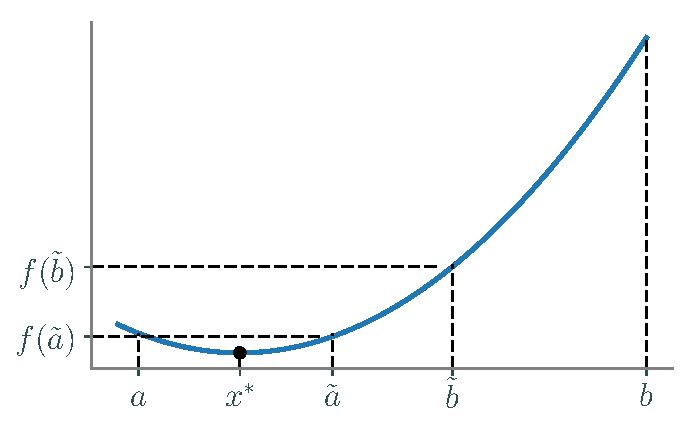
\includegraphics[width=.7\textwidth]{figures/golden_section.pdf}
    \caption{The unimodal $f:[a,b]\rightarrow\mathbb{R}$ can be minimized with a golden section search.
    For the first iteration, $f(\tilde{a}) < f(\tilde{b})$, so $x^* \in [a, \tilde{b}]$.
    New values of $\tilde{a}$ and $\tilde{b}$ are then calculated from this new, smaller interval.}
    \label{fig:1dopt-golden-unimodal}
\end{figure}

\begin{algorithm}[H]
\begin{algorithmic}[1]
\Procedure{golden\_section}{$f$,\ $a$,\ $b$,\ \li{tol},\ \li{maxiter}}
   \State $x_0 \gets (a + b)/2$
        \Comment{Set the initial minimizer approximation as the interval midpoint.}
   \State $\varphi = (1+\sqrt{5})/2$
        % \Comment{Set $\varphi$.}
   \For{$i=1,2,\dots,$\ \li{maxiter}}
        \Comment Iterate only \li{maxiter} times at most.
        \State $c \gets (b - a)/\varphi$
        \State $\tilde{a} \gets b - c$
            % \Comment{Set $\tilde{a}$.}
        \State $\tilde{b} \gets a + c$
            % \Comment{Set $\tilde{b}$. }
        \If{$f(\tilde{a}) \leq f(\tilde{b})$}
            \Comment{Get new boundaries for the search interval.}
            \State $b \gets \tilde{b}$
         \Else{}
            \State $a \gets \tilde{a}$
                \EndIf
        \State $x_1 \gets (a + b)/2$
            \Comment{Set the minimizer approximation as the interval midpoint.}
        \If{$|x_0-x_1| <$ \li{tol}}
              \State \texttt{break}
                \Comment{Stop iterating if the approximation stops changing enough.}
       \EndIf
        \State $x_0 \gets x_1$
   \EndFor
   \State \pseudoli{return} $x_1$
\EndProcedure
\end{algorithmic}
\caption{The Golden Section Search}
\label{Alg:Golden-Section-Search}
\end{algorithm}

\begin{problem}{Implement golden search.}
Write a function that accepts a function $f:\mathbb{R}\rightarrow\mathbb{R}$, interval limits $a$ and $b$, a stopping tolerance \li{tol}, and a maximum number of iterations \li{maxiter}.
Use Algorithm \ref{Alg:Golden-Section-Search} to implement the golden section search.
Return the approximate minimizer $x^*$, whether or not the algorithm converged (\li{true} or \li{false}), and the number of iterations computed.

Test your function by minimizing $f(x) = e^x - 4x$ on the interval $[0, 3]$, then plotting the function and the computed minimizer together.
Also compare your results to SciPy's golden section search, \li{scipy.optimize.golden()}.

\begin{lstlisting}
>>> from scipy import optimize as opt
>>> import numpy as np

>>> f = lambda x : np.exp(x) - 4*x
>>> opt.golden(f, brack=(0,3), tol=.001)
1.3862578679031485              # ln(4) is the minimizer.
\end{lstlisting}
\label{prob:golden-section-search}
\end{problem}

\section*{Newton's Method} % ==================================================

\emph{Newton's method} is an important root-finding algorithm that can also be used for optimization.
Given $f:\mathbb{R}\rightarrow\mathbb{R}$ and a good initial guess $x_0$, the sequence $(x_k)_{k=1}^\infty$ generated by the recursive rule
\[
x_{k+1} = x_k - \frac{f(x_k)}{f'(x_k)}
\]
converges to a point $\bar{x}$ satisfying $f(\bar{x}) = 0$.
The first-order necessary conditions from elementary calculus state that if $f$ is differentiable, then its derivative evaluates to zero at each of its local minima and maxima.
Therefore using Newton's method to find the zeros of $f'$ is a way to identify potential minima or maxima of $f$.
Specifically, starting with an initial guess $x_0$, set
\begin{equation}
x_{k+1} = x_k - \frac{f'(x_k)}{f''(x_k)}
\label{eq:1dopt-newton}
\end{equation}
and iterate until $|x_k - x_{k-1}|$ is satisfactorily small.
Note that this procedure does not use the actual function $f$ at all, but it requires many evaluations of its first and second derivatives.
As a result, Newton's method converges in few iterations, but it can be computationally expensive.

Each step of \eqref{eq:1dopt-newton} can be thought of approximating the objective function $f$ by a quadratic function $q$ and finding its unique extrema.
That is, we first approximate $f$ with its second-degree Taylor polynomial centered at $x_k$.
\[
q(x) = f(x_k) + f'(x_k) (x - x_k) + \frac{1}{2} f''(x_k) (x - x_k)^2
\]
This quadratic function satisfies $q(x_k) = f(x_k)$ and matches $f$ fairly well close to $x_k$.
Thus the optimizer of $q$ is a reasonable guess for an optimizer of $f$.
To compute that optimizer, solve $q'(x) = 0$.
\[
0 = q'(x) = f'(x_k) + f''(x_k)(x - x_k)
\qquad\Longrightarrow\qquad
x = x_k - \frac{f'(x_k)}{f''(x_k)}
\]
This agrees with \eqref{eq:1dopt-newton} using $x_{k+1}$ for $x$.
See Figure \ref{fig:1dopt-quadratic-newton}.

\begin{figure}[H]
\centering
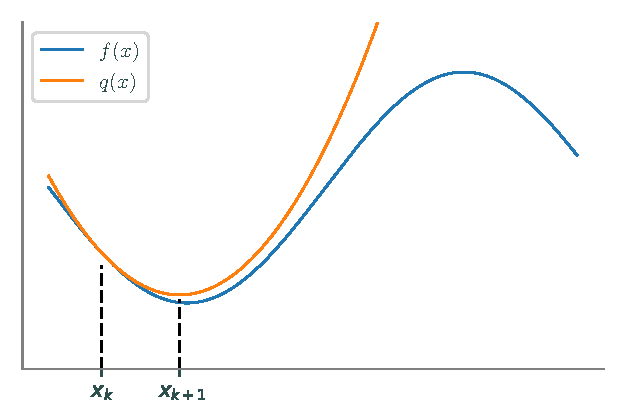
\includegraphics[width = .7 \textwidth]{figures/quad_approx.pdf}
\caption{A quadratic approximation of $f$ at $x_k$.
The minimizer $x_{k+1}$ of $q$ is close to the minimizer of $f$.
}
\label{fig:1dopt-quadratic-newton}
\end{figure}

Newton's method for optimization works well to locate minima when $f''(x) > 0$ on the entire domain.
However, it may fail to converge to a minimizer if $f''(x) \le 0$ for some portion of the domain.
If $f$ is not unimodal, the initial guess $x_0$ must be sufficiently close to a local minimizer $x^*$ in order to converge.

\begin{problem}{Newton's method for optimization}{}
Let $f:\mathbb{R}\rightarrow\mathbb{R}$.
Write a function that accepts $f'$, $f''$, a starting point $x_0$, a stopping tolerance \li{tol}, and a maximum number of iterations \li{maxiter}.
Implement Newton's method using \eqref{eq:1dopt-newton} to locate a local optimizer.
Return the approximate optimizer, whether or not the algorithm converged, and the number of iterations computed.

Test your function by minimizing $f(x) = x^2 + \sin(5x)$ with an initial guess of $x_0 = 0$.
Compare your results to \li{scipy.optimize.newton()}, which implements the root-finding version of Newton's method.
\begin{lstlisting}
>>> df = lambda x : 2*x + 5*np.cos(5*x)
>>> d2f = lambda x : 2 - 25*np.sin(5*x)
>>> opt.newton(df, x0=0, fprime=d2f, tol=1e-10, maxiter=500)
-1.4473142236328096
\end{lstlisting}
Note that other initial guesses can yield different minima for this function.
\end{problem}


\paragraph{Convervence of Newton's Method}

We consider the function $f(x) = e^x + e^{-x}$.

\begin{tabular}{lrrrrr}
\toprule
{} &           $x$ &      $f(x)$ &  $f^\prime(x)$ &  $|x^k - x^{k-1}|$ &  $\frac{|x^ k - x^{k-1}|}{|x^{k-1} - x^{k-2}|}$ \\
\midrule
0 &  6.100000e+00 &  445.860013 &   4.458555e+02 &                NaN &                                            NaN \\
0 &  5.100010e+00 &  164.029654 &   1.640175e+02 &       9.999899e-01 &                                            NaN \\
0 &  4.100084e+00 &   60.361952 &   6.032881e+01 &       9.999257e-01 &                                   9.999357e-01 \\
0 &  3.100633e+00 &   22.257038 &   2.216700e+01 &       9.994509e-01 &                                   9.995252e-01 \\
0 &  2.104679e+00 &    8.326354 &   8.082584e+00 &       9.959545e-01 &                                   9.965016e-01 \\
0 &  1.133956e+00 &    3.429685 &   2.786169e+00 &       9.707231e-01 &                                   9.746662e-01 \\
0 &  3.215870e-01 &    2.104313 &   6.543175e-01 &       8.123688e-01 &                                   8.368697e-01 \\
0 &  1.064582e-02 &    2.000113 &   2.129203e-02 &       3.109412e-01 &                                   3.827587e-01 \\
0 &  4.021572e-07 &    2.000000 &   8.043143e-07 &       1.064541e-02 &                                   3.423609e-02 \\
0 & -6.935643e-17 &    2.000000 &  -1.110223e-16 &       4.021572e-07 &                                   3.777751e-05 \\
0 & -1.384528e-17 &    2.000000 &   0.000000e+00 &       5.551115e-17 &                                   1.380335e-10 \\
0 & -1.384528e-17 &    2.000000 &   0.000000e+00 &       0.000000e+00 &                                   0.000000e+00\\
\hline
\end{tabular}

\subsection*{The Secant Method} % ---------------------------------------------

The second derivative of an objective function is not always known or may be prohibitively expensive to evaluate.
The \emph{secant method} solves this problem by numerically approximating the second derivative with a difference quotient.
\[
f''(x) \approx \frac{f'(x + h) - f'(x)}{h}
\]
Selecting $x = x_k$ and $h = x_{k-1} - x_k$ gives the following approximation.
\begin{equation}
f''(x_k) \approx \frac{f'(x_k + x_{k-1} - x_k) - f'(x_k)}{x_{k-1} - x_k}
= \frac{f(x_k) - f'(x_{k-1})}{x_k - x_{k-1}}
\label{eq:1dopt-secant-approx}
\end{equation}
% The \emph{Secant method} approximates it using secant lines, or in other words, the rate of change between points.
Inserting \eqref{eq:1dopt-secant-approx} into \eqref{eq:1dopt-newton} results in the complete secant method formula.
\begin{equation}
x_{k+1}
= x_k - \frac{x_k - x_{k-1}}{f'(x_k) - f'(x_{k-1})}f'(x_k)
= \frac{x_{k-1}f'(x_k) - x_{k}f'(x_{k-1})}{f'(x_k) - f'(x_{k-1})}
\label{eq:1dopt-secant-method}
\end{equation}
Notice that this recurrence relation requires two previous points (both $x_{k}$ and $x_{k-1}$) to calculate the next estimate.
This method converges superlinearly---slower than Newton's method, but faster than the golden section search---with convergence criteria similar to Newton's method.

\begin{problem}{Implement secant method}{}
Write a function that accepts a first derivative $f'$, starting points $x_0$ and $x_1$, a stopping tolerance \li{tol}, and a maximum of iterations \li{maxiter}.
Use \eqref{eq:1dopt-secant-method} to implement the Secant method.
Try to make as few computations as possible by only computing $f'(x_k)$ once for each $k$.
Return the minimizer approximation, whether or not the algorithm converged, and the number of iterations computed.

Test your code with the function $f(x) = x^2 + \sin(x) + \sin(10x)$ and with initial guesses of $x_0 = 0$ and $x_1 = -1$.
Plot your answer with the graph of the function.
Also compare your results to \li{scipy.optimize.newton()}; without providing the \li{fprime} argument, this function uses the secant method.
% Note that this function is highly sensitive to the starting point, which is why it is not as helpful to compare your function with SciPy's method.
However, it still only takes in one initial condition, so it may converge to a different local minimum than your function.

\begin{lstlisting}
>>> df = lambda x: 2*x + np.cos(x) + 10*np.cos(10*x)
>>> opt.newton(df, x0=0, tol=1e-10, maxiter=500)
-3.2149595174761636
\end{lstlisting}
\end{problem}

\section*{Descent Methods} % ==================================================

Consider now a function $f:\mathbb{R}^n\rightarrow\mathbb{R}$.
% Minimizing $f$ is a \emph{high-dimensional optimization problem} because the domain of $f$ is $\mathbb{R}^n$ instead of $\mathbb{R}$.
\emph{Descent methods}, also called \emph{line search methods}, are optimization algorithms that create a convergent sequence $(x_k)_{k=1}^\infty$ by the following rule.
\begin{equation}
\x_{k+1} = \x_k + \alpha_k \textbf{p}_k
\end{equation}
Here $\alpha_k \in \mathbb{R}$ is called the \emph{step size} and $\textbf{p}_k \in \mathbb{R}^n$ is called the \emph{search direction}.
The choice of $\textbf{p}_k$ is usually what distinguishes an algorithm;
in the one-dimensional case ($n = 1$), $p_k = f'(x_k)/f''(x_k)$ results in Newton's method, and using the approximation in \eqref{eq:1dopt-secant-approx} results in the secant method.

To be effective, a descent method must also use a good step size $\alpha_k$.
If $\alpha_k$  is too large, the method may repeatedly overstep the minimum; if $\alpha_k$ is too small, the method may converge extremely slowly.
See Figure \ref{fig:1dopt-overstep}.

\begin{figure}[H]
    \centering
    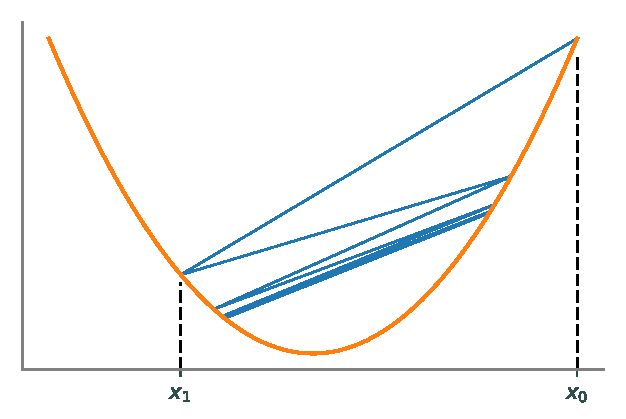
\includegraphics[width=.7\textwidth]{figures/large_alpha.pdf}
    \caption{If the step size $\alpha_k$ is too large, a descent method may repeatedly overstep the minimizer.}
    \label{fig:1dopt-overstep}
\end{figure}

Given a search direction $\textbf{p}_k$, the best step size $\alpha_k$ minimizes the function $\phi_k(\alpha) = f(\x_k + \alpha\textbf{p}_k)$.
Since $f$ is scalar-valued, $\phi_k:\mathbb{R}\rightarrow\mathbb{R}$, so any of the optimization methods discussed previously can be used to minimize $\phi_k$.
However, computing the best $\alpha_k$ at every iteration is not always practical.
 % especially since computing a good $\mathbf{p}_k$ is generally more critical.
Instead, some methods use a cheap routine to compute a step size that may not be optimal, but which is good enough.
% These methods do not seek to minimize $\phi_k(\alpha)$, but instead seek to sufficiently decrease it.
The most common approach is to find an $\alpha_k$ that satisfies the \emph{Wolfe conditions}:
\begin{align}
&f(\textbf{x}_k + \alpha_k \textbf{p}_k) \leq f(\textbf{x}_k) + c_1\alpha_k Df(\textbf{x}_k)\trp \textbf{p}_k
\label{eq:1dopt-wolfe-armijo}
\\
& - Df(\textbf{x}_k + \alpha_k \textbf{p}_k)\trp \textbf{p}_k \leq -c_2 Df(\textbf{x}_k)\trp \textbf{p}_k
\label{eq:1dopt-wolfe-curvature}
\end{align}
where $0 < c1 < c2 < 1$ (for the  best results, choose $c1 << c2$).
The condition \eqref{eq:1dopt-wolfe-armijo} is also called the \emph{Armijo rule} and ensures that the step decreases $f$.
However, this condition is not enough on its own.
By Taylor's theorem,
\[
f(\textbf{x}_k + \alpha_k \textbf{p}_k) = f(\textbf{x}_k) + \alpha_k Df(\textbf{x}_k)\trp \textbf{p}_k + \mathcal{O}(\alpha_k^2).
\]
Thus, a very small $\alpha_k$ will always satisfy \eqref{eq:1dopt-wolfe-armijo} since $Df(\textbf{x}_k)\trp\textbf{p}_k < 0$ (as $\textbf{p}_k$ is a descent direction).
The condition \eqref{eq:1dopt-wolfe-curvature}, called the \emph{curvature condition}, ensures that the $\alpha_k$ is large enough for the algorithm to make significant progress.

It is possible to find an $\alpha_k$ that satisfies the Wolfe conditions, but that is far from the minimizer of $\phi_k(\alpha)$.
The \emph{strong Wolfe conditions} modify \eqref{eq:1dopt-wolfe-curvature} to ensure that $\alpha_k$ is near the minimizer.
\[
| Df(\textbf{x}_k + \alpha_k \textbf{p}_k)\trp \textbf{p}_k| \leq c_2| Df(\textbf{x}_k)\trp \textbf{p}_k|
\]
The \emph{Armijo--Goldstein conditions} provide another alternative to \eqref{eq:1dopt-wolfe-curvature}:
\[
f(\textbf{x}_k) + (1 - c)\alpha_k Df(\textbf{x}_k)\trp \textbf{p}_k \leq f(\textbf{x}_k + \alpha_k\textbf{p}_k) \leq f(\textbf{x}_k) + c\alpha_k Df(\textbf{x}_k)\trp\textbf{p}_k,
\]
where $0 < c < 1$.
These conditions are very similar to the Wolfe conditions (the right inequality is \eqref{eq:1dopt-wolfe-armijo}), but they do not require the calculation of the directional derivative $ Df(\textbf{x}_k + \alpha_k \textbf{p}_k)\trp\textbf{p}_k$.
% They perform as well as the Wolfe conditions in most situations, but are not well-matched for quasi-Newton methods with positive definite Hessians. % ?

\subsubsection*{Backtracking}

A \emph{backtracking line search} is a simple strategy for choosing an acceptable step size $\alpha_k$: start with an fairly large initial step size $\alpha$, then repeatedly scale it down by a factor $\rho$ until the desired conditions are satisfied.
The following algorithm only requires $\alpha$ to satisfy \eqref{eq:1dopt-wolfe-armijo}.
This is usually sufficient, but if it finds $\alpha$'s that are too small, the algorithm can be modified to satisfy \eqref{eq:1dopt-wolfe-curvature} or one of its variants.

\begin{algorithm}[H]
\begin{algorithmic}[1]
\Procedure{backtracking}{$f$,\ $Df$,\ $\x_k$,\ $\mathbf{p}_k$,\ $\alpha$,\ $\rho$,\ $c$}
    \State \texttt{Dfp} $\gets Df(\x_k)\trp\mathbf{p}_k$
        \Comment{Compute these values only once.}
    \State \texttt{fx} $\gets f(\x_k)$
    \While{$\big(f(\x_k + \alpha\mathbf{p}_k) >$ \texttt{fx} $+\ c\alpha$\texttt{Dfp}$\big)$}
        \State $\alpha \gets \rho\alpha$
    \EndWhile
    \Return $\alpha$
\EndProcedure
\end{algorithmic}
\caption{Backtracking using the Armijo Rule}
\label{Alg:opt1d-backtracking}
\end{algorithm}

\begin{problem}{Implement the backtracking method}{}
Write a function that accepts a function $f:\mathbb{R}^n\rightarrow\mathbb{R}$, its derivative $Df:\mathbb{R}^n\rightarrow\mathbb{R}^n$, an approximate minimizer $\x_k$, a search direction $\textbf{p}_k$, an initial step length $\alpha$, and parameters $\rho$ and $c$.
Implement the backtracking method of Algorithm \ref{Alg:opt1d-backtracking}.
Return the computed step size.

The functions $f$ and $Df$ should both accept 1-D NumPy arrays of length $n$.
For example, if $f(x,y,z) = x^2 + y^2 + z^2$, then $f$ and $Df$ could be defined as follows.
\begin{lstlisting}
>>> f = lambda x: x[0]**2 + x[1]**2 + x[2]**2
>>> Df = lambda x: np.array([2*x[0], 2*x[1], 2*x[2]])
\end{lstlisting}

SciPy's \li{scipy.optimize.linesearch.scalar_search_armijo()} finds an acceptable step size using the Armijo rule.
It may not give the exact answer as your implementation since it decreases $\alpha$ differently, but the answers should be similar.
\begin{lstlisting}
>>> from scipy.optimize import linesearch
>>> from autograd import numpy as anp
>>> from autograd import grad

# Get a step size for f(x,y,z) = x^2 + y^2 + z^2.
>>> f = lambda x: x[0]**2 + x[1]**2 + x[2]**2
>>> x = anp.array([150., .03, 40.])         # Current minimizer guesss.
>>> p = anp.array([-.5, -100., -4.5])       # Current search direction.
>>> phi = lambda alpha: f(x + alpha*p)      # Define phi(alpha).
>>> dphi = grad(phi)
>>> alpha, _ = linesearch.scalar_search_armijo(phi, phi(0.), dphi(0.))
\end{lstlisting}
\end{problem}

\begin{comment} % This is a little too confusing and needs revision if it's going to be in print.

\newpage

\section*{Additional Material} % ==============================================

\subsection*{Golden Search Derivations} % -------------------------------------

The ratio of the lengths of $[a, \tilde{a}]$ and $[\tilde{a}, b]$ is the same as the ratio between the lengths of $[\tilde{a}, b]$ and $[a, b]$ as follows:
\begin{align*}
\frac{\tilde{a}-a}{b-\tilde{a}} &= \frac{(b-a)(1-\frac{1}{\varphi})}{b-b+\frac{b-a}{\varphi}} \\
&= \varphi(1-\frac{1}{\varphi}) \\
\frac{b-\tilde{a}}{b-a} &= \frac{1}{\varphi}
\end{align*}
As one of the properties of the golden ratio states that $\frac{1}{\varphi^2} = 1 - \frac{1}{\varphi}$, they are equal.

Chosing the test points according to the golden ratio saves on computations.
For example, consider the case where $f(\tilde{a}) > f(\tilde{b})$ and label $a_0 = a$ and $a_1 = \tilde{a}$.
Thus, $x^* \in [\tilde{a}, b]$ and for the next iteration
\begin{align*}
\tilde{a_1} &= b - \frac{b - a_1}{\varphi} \\
&= b - \frac{b - b + \frac{b - a_0}{\varphi}}{\varphi}\\
&= b - \frac{b - a_0}{\varphi^2}\\
&= a_0 + \frac{b - a_0}{\varphi}\\
&= \tilde{b}
\end{align*}
Therefore, the next $\tilde{a}$ is the previous $\tilde{b}$.
Similarly, if $f(\tilde{a}) < f(\tilde{b})$, then the next $\tilde{b}$ will be the previous $\tilde{a}$.
\end{comment}
